\section{Organization of the project}\label{sec:organization}

Before running any script, the project must be opened. With the MATLAB console
placed into the project folder, the project can be opened by typing (note the
dot):
\begin{verbatim}
> openProject .
\end{verbatim}
Alternatively, the project can be opened from the MATLAB GUI by using menus.

When the project is opened, the MATLAB path is automatically updated in order
to include all the source folders of the project.

The project is divided in the following folders:
\begin{description}
	\item[data/] contains the data saved by stages after execution. See
		\secref{subsec:stages}.
	\item[diaries/] contains diaries of execution of the scripts.
	\item[figures/] contains exported figures.
	\item[resources/] contains MATLAB's project resources. Nothing useful
		here.
	\item[src/] contains all source code files. It has the following
		subdirectories and files:
		\begin{description}
			\item[scripts/] contains the scripts usually run from
				MATLAB console.
			\item[stages/] contains stages used to build the
				pipelines used by scripts (see
				\secref{subsec:stages}).
			\item[cnndefs/] contains various CNN defnitions used in
				\chref{ch:cnn}.
			\item[rnndefs/] contains various RNN defnitions used in
				\chref{ch:rnn}.
			\item[mamdani.fis] is the Mamdani FIS developed in
				\chref{ch:fuzzy}.
			\item[startup.m] that it is run automatically when the
				project is opened. It just sets up some global
				variables.
			\item[diaryon.m] contains an utility function used to
				log the output of a script. It supports
				rotation of the diaries if a diary with the
				same name already exists.
			\item[exportfigure.m] contains the function used to
				export vectorial graphics to PDF.
			\item[other files] are used to define and run stages
				(see \secref{subsec:stages}).
		\end{description}
\end{description}

\subsection{Stages and pipelines}\label{subsec:stages}

Development of intelligent systems can be often seen as a ``pipelined'' process
going through different ``stages''. For example, if you need to train a
multi-layer perceptron, you need to:
\begin{enumerate}
	\item load data;
	\item perform data augmentation;
	\item extract features and targets;
	\item normalize features;
	\item train the network.
\end{enumerate}
Those steps are performed one after another. This can be seen as data passing
through a pipeline. Scripts in the project (\code{src/scripts/} folder) often
build and run a pipeline composed by many stages (\code{src/stages/} folder).

A stage is simply a function that takes input from other stages and, possibly,
some additional parameters. When a stage is executed, the result is saved in a
file under the \code{data/} folder. The next time the stage needs to be
executed, the result is loaded from the file instead of being recomputed
(unless explicitly requested).

Stages are defined as instances of the class \code{Stage} and executed by the
\code{runstages} function.

To understand how stages are executed consider, as an example, the pipeline
shown in \lstref{lst:pipelineexample}. The pipeline can be also seen as an
acyclic directed graph as shown in \figref{fig:pipelineexample}. Description of
what each stage does can be found in \chref{ch:dataset}.

\lstinputlisting[language={matlab}, label={lst:pipelineexample},
style={Matlab-editor}, basicstyle={\scriptsize\ttfamily}, caption={A simple
pipeline, composed by 5 stages. Used only as an example.}]{pipelineexample.m}

\begin{figure}[htbp]
	\centering
	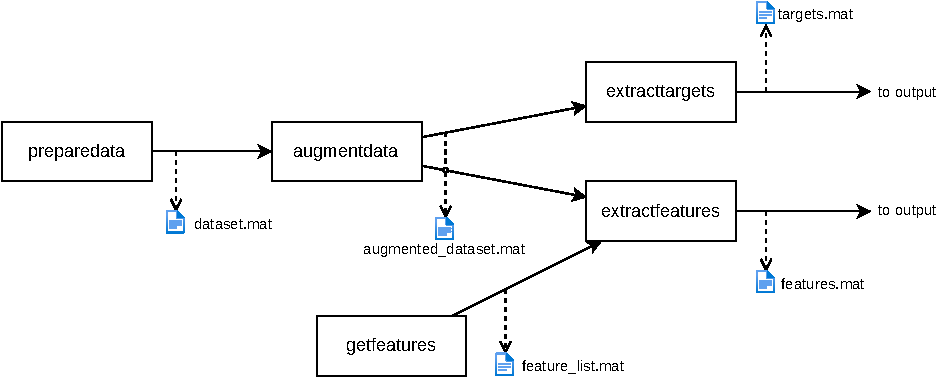
\includegraphics[width=\textwidth]{pipelineexample}
	\caption{Graphical representation of the example pipeline defined in
	\lstref{lst:pipelineexample}.}\label{fig:pipelineexample}
\end{figure}

When the \code{runstages} function is called for the first time (no cached data
available), the pipeline is executed as follows:
\begin{enumerate}
	\item The \code{preparedata} stage is executed, meaning that the
		function defined in \code{src/stages/preparedata.m} is called.
		The result, a structure containing the entire dataset, is saved
		in file \code{dataset.mat}.
	\item The \code{augmentdata} stage is executed. This stage has
		\code{preparedata} as input stage. The output of the
		\code{preparedata} stage is automatically passed as argument to
		the function which implements the \code{augmentdata} stage,
		defined in \code{src/stages/augmentdata.m}. Result of this
		stage is also saved (as for every stage).
	\item The \code{getfeatures} stage is executed. It's output is used as
		input in the next stage.
	\item The \code{extractfeatures} stage is executed. We have 2 input
		stages here: the first parameter passed to the function will be
		a structure containing the output of both input stages (fields
		of structure are named after the input stages' names).
	\item The \code{extracttargets} stage is executed, with a single input
		stage.
	\item The \code{runstages} function returns a structure containing a
		field for each stage explicitly requested via actual arguments
		\idest{\code{extractfeatures} and \code{extracttargets}}. So
		that, for example, the output of the execution of stage
		\code{extractfeatures} can be accessed, after the call to
		\code{runstages}, as \code{result.extractfeatures}.
\end{enumerate}

When cached data are available, stages are usually not executed. More
precisely, it depends on the value of the \code{RunPolicy} property of the
\code{Stage} class. The default value is \code{RunPolicy.OLD}, meaning that the
stage is executed only if no cached data are available or if cached data is
outdated. For details, see comments in files \code{RunPolicy.m}, \code{Stage.m}
and \code{runstages.m}.

This architecture was build in order to avoid having to worry, during
development, to save and load the data of the various intermediate steps.

Note that, to save some space, I've removed most of the files from the
\code{data} directory. I've left there only the most important files
\exgratia{those containing the trained intelligent systems}.
